\input{style/settings}
\input{style/short_commands}
\pagestyle{fancy}
\fancyhf{}
\fancyhead[R]{página\;\thepage/\pageref{LastPage}}
\fancyhead[L]{Osvaldo Uriel Calderón Dorantes}
\fancyfoot[L]{Imagenología Biomédica}
\fancyfoot[R]{Facultad de Ciencias, UNAM 
\includegraphics[scale=0.13]{style/Sheikah.pdf}}
\fancypagestyle{plain}{
  \fancyfoot[C]{}
}
\makeatletter
\def\@seccntformat#1{%
  \expandafter\ifx\csname c@#1\endcsname\c@section\else
  \csname the#1\endcsname\quad
  \fi}
\makeatother
%%%%%%%%%%%%%%%%%%%%%%%%%%%%%%%%%%%%%%%%%%%%%%%%%%%%%%%
%%%%%%%%%%%%%%%%%%%%%%%%%%%%%%%%%%%%%%%%%%%%%%%%%%%%%%%%%%%
\begin{document}
\begin{flushleft}
Osvaldo Uriel Calderón Dorantes, \hfill Imagenología Biomédica\\
316005171 \hfill osvaldo13576@ciencias.unam  \\
Facultad de Ciencias\\
\underline{Universidad Nacional Autónoma de México}
\end{flushleft}

\begin{flushright}\vspace{-5mm}

\includegraphics[height=1.5cm]{style/logo.pdf}
\end{flushright}
 
\begin{center}\vspace{-1cm}
\textbf{ \large \customfont{Tarea 2\\
Módulo RADIODIAGNÓSTICO}}\\
\today
\end{center}
%\medskip\hrule\medskip
%%%%%%%%%%%%%%%%%%%%%%%%%%%%%%%%%%%%%%%%%%%%%%%%
%{\small \textbf{Nota: A las unidades las pondré dentro de corchetes \ec{[\tx{unidad}]} para no confundir entre variables y realizar el análisis dimensional fácilmente.}}
\medskip\hrule\bigskip

\newlength{\strutheight}
\settoheight{\strutheight}{\strut}


\begin{enumerate}[1.]
\item ¿En qué consiste la CT cardíaca?



\begin{figure}[!ht]
\centering
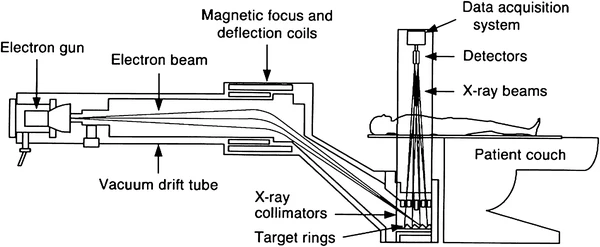
\includegraphics[width=0.7\textwidth]{./figuras/40134_2012_5_Fig13_HTML.png}
\caption{Esquema para de un CT de haz de electrones sin piezas móviles. La figura se recuperó de \citep{Flohr}.}
\label{p1:ct}
\end{figure}

El estudio de la CT cardíaca introduce la quinta generación de CT \citep{IM}, la cual viene con mejoras en tiempo de adquisición ultrarápidas, ya que se toma en cuenta que se tiene alrededor de 60 latidos por minuto y 1 segundo de duración del ciclo cardíaco y para tener una imagen estática del corazón se requería una ventada de tiempo de adquisición de 100 milisegundos o incluso menos. Con ello se desarrolló en 1984 la CT de haz de electrones (EBCT)  \citep{jerro}.


En la figura \ref{p1:ct} se observa el funcionamiento del sistema EBCT. Este sistema consta de un tubo de rayos X estacionario y un anillo de detectores de tungsteno también estacionario, el mecanismo es el siguiente: El cañón de electrones emite un haz de electrones acelerados con un potencial de aproximadamente \ec{120\;kV}  y son desviados magnéticamente por una bobina magnética, esta desviación barre el haz y lo dirige hacia el anillo, provocando la generación de rayos X en un arco de \ec{210^\circ}  \citep{Flohr,jerro}. 


\item  ¿En qué consiste la CT helicoidal?


\begin{figure}[!ht]
  \centering
  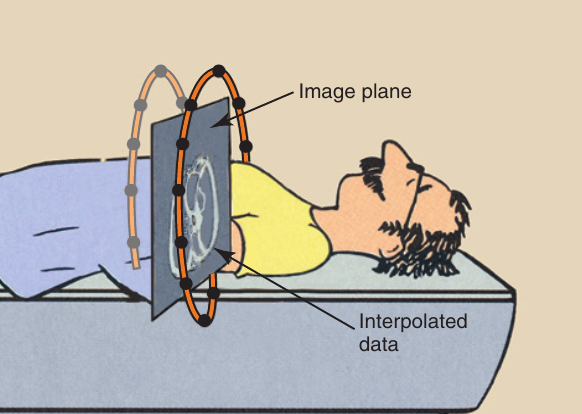
\includegraphics[width=0.5\textwidth]{./figuras/p2_ct.png}
  \caption{Se realiza un muestreo de los datos de manera continua y se realiza una interpolación (estimación de un valor dado dos datos conocidos) de estos para reconstruir la imagen en cualquier plano transversal. La figura se recuperó de \citep{stewart}.}
  \label{p2:ct}
  \end{figure}

Se trata de una sexta generación de CT \citep{IM}, la cual puede verse como si el paciente se moviera a lo largo del eje horizontal a medida que el tubo de rayos X gira alrededor de éste, como se muestra en la figura \ref{p2:ct}, entonces el haz de rayos X sigue una trayectoria helicoidal \citep{stewart}. 

Se toma en cuenta el concepto Pitch, el cual se define como se establece en la ec. \ref{ec:p2}, entonces, si tenemos que la cama del paciente se mueve \ec{8\;mm} y el ancho del haz es de \ec{5\;mm}, entonces el pitch es de \ec{8\;mm/5\;mm=1.6}, la importancia de este concepto en la imagenología es que al aumentar el pitch, tendremos una reducción del tiempo de exploración y dosis al paciente, además, se obtiene un aumento del perfil de sensibilidad de corte y el ancho de corte efectivo \citep{stewart,jerro}.



\eq{ec:p2}{\tx{Pitch}=\dfrac{\tx{Movimiento de la cama cada }360^\circ}{\tx{Ancho del haz}}}

Para reconstruir las imágenes empleando este CT, se usa la interpolación de datos de la proyección a lo largo del eje del paciente en una posición seleccionada de interés, ya que la fuente de rayos X se ha desplazado de forma helicoidal a lo largo del paciente  y los algoritmos de reconstrucción suponen que la fuente de rayos X realiza una trayectoria circular y no una helicoidal.









\item ¿En qué consiste la CT multicorte?

\begin{figure}[!ht]
  \centering
  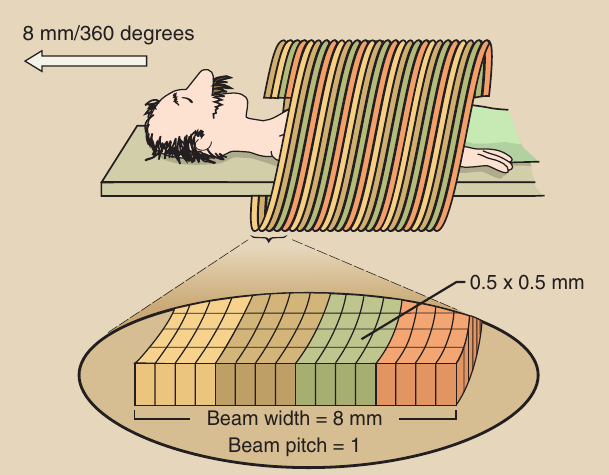
\includegraphics[width=0.6\textwidth]{./figuras/p3_ct.png}
  \caption{Se cuenta con una matriz de detectores de 16 detectores con un ancho de \ec{0.5\;mm} y un ancho de colimado de \ec{8\;mm} dando un pitch de \ec{0.5\times16/8=1}. La figura se recuperó de \citep{stewart}.}
  \label{p3:ct}
  \end{figure}


Es la séptima generación de CT \citep{IM}, la CT multicorte hace uso de múltiples conjuntos de detectores para emplear una porción más amplia del haz de rayos X durante la adquisición de datos, consisten de una forma de CT  helicoidal donde se hace uso de múltiples anillos de detectores para escanear múltiples cortes del cuerpo durante cada rotación. El grosor de la sección se determina por el ancho del detector y no por el sistema de colimación, es decir, se pueden combinar cuatro filas de detectores para registrar simultáneamente cuatro secciones adyacentes en una sola rotación y que el ancho sea la suma de los anchos de cada detector. La ventaja de esta tecnología es que hace un mejor uso de la salida del haz del tubo de rayos X lo cual disminuye la carga térmica, además, mejora el tiempo de escaneo y reduce los artefactos debido al movimiento \citep{jerro,russ}.


\pagebreak

\item ¿Qué es un sinograma? ¿Por qué nos interesa estudiar un sinograma en imagenología?


\begin{figure}[!ht]
  \centering
  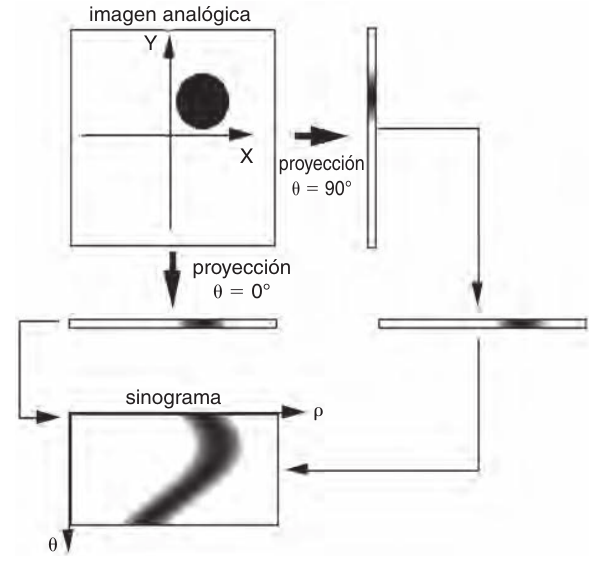
\includegraphics[width=0.5\textwidth]{./figuras/p4_sino.png}
  \caption{Sinograma de una imagen analógica. La figura se recuperó de \citep{andre}.}
  \label{p4:sino}
  \end{figure}

Un sinograma son los datos resultantes a los cuales se les ha aplicado la transformada de Radón, de forma práctica un camino para llegar a un sinograma es tomar las proyecciones y colocándolas como columnas enotra matriz. De acuerdo a la figura \ref{p4:sino}, si tomamos la proyección para cada ángulo tendremos una una distribución, las cuales se pueden superponer en caso de tener más objetos, entonces se puede construir una gráfica del ángulo contra la distribución en esa proyección. 

La importancia en la imagenología es que puede detectar el movimiento del paciente, estos movimientos resultan en grandes artefactos cuando se reconstruye la imagen \citep{smith}.

\begin{figure}[!ht]
  \centering
  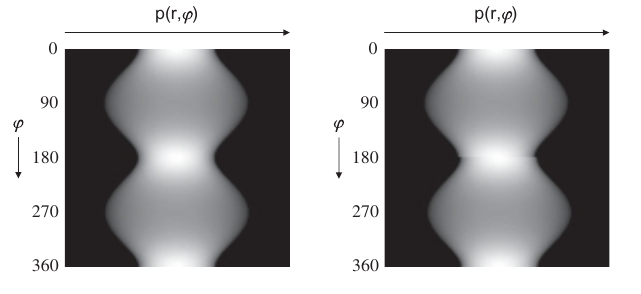
\includegraphics[width=0.7\textwidth]{./figuras/p4_2.png}
  \caption{El sinograma izquierdo de un objeto que permaneció estático durante el escaneo, el de la derecha realizó un movimiento a la mitad del procedimiento provando un desplazamiento del sinograma. La figura se recuperó de \citep{smith}.}
  \label{p4:sino2}
  \end{figure}

\pagebreak

\item Utiliza tu número de cuenta para construir una matriz de 3x3. Obtén las proyecciones y la matriz de retroproyección (mostrar cada paso realizado)

Tenemos la matriz de proyección con mi número de cuenta: \ec{316005171}

\ecc{
X=  
\begin{bmatrix}
  3 & 1 & 6\\
  0 & 0 & 5\\
  1 & 7 & 1
  \end{bmatrix}}

  \subsection{Primer paso}

  Tomamos las proyecciones de las columnas y formamos la matriz de proyección \ec{a}:
  \ecc{
a=  
\begin{bmatrix}
  \frac{4}{3} & \frac{8}{3} & \frac{12}{3}\\ \\ 
  \frac{4}{3} & \frac{8}{3} & \frac{12}{3}\\ \\
  \frac{4}{3} & \frac{4}{3} & \frac{12}{3}
  \end{bmatrix}}

\subsection{Segundo paso}
Construimos una matriz \ec{b} sumando los valores de la filas de la matriz \ec{X}
\ecc{
b=  
\begin{bmatrix}
  \frac{10}{3} & \frac{10}{3} & \frac{10}{3}\\ \\ 
  \frac{5}{3} & \frac{5}{3} & \frac{5}{3}\\ \\
  \frac{9}{3} & \frac{9}{3} & \frac{9}{3}
  \end{bmatrix}}

  \subsection{Tercer paso}
Consideramos la proyección angular, las diagonales, de izquierda a derecha
\ecc{
  c=
\begin{bmatrix}
  \frac{3}{1} & \frac{1}{2} & \frac{7}{3}\\ \\ 
  \frac{1}{2} & \frac{7}{3} & \frac{12}{2}\\ \\
  \frac{7}{3} & \frac{12}{2} & \frac{1}{1}
  \end{bmatrix}}


\subsection{Cuarto paso}
Como el paso anterior, tomamos la suma de diagonales de derecha a izquierda
\ecc{
  d=
\begin{bmatrix}
  \frac{4}{3} & \frac{6}{2} & \frac{6}{1}\\ \\ 
  \frac{7}{2} & \frac{4}{3} & \frac{6}{2}\\ \\
  \frac{1}{1} & \frac{7}{2} & \frac{4}{3}
  \end{bmatrix}}

\pagebreak

\subsection{Quinto paso}
Obtenemos la matriz de retroproyección al sumar las matrices \ec{a}, \ec{b}, \ec{c} y \ec{d}.
\al{M&=a+b+c+d\\
&=\begin{bmatrix}
  \frac{4}{3} & \frac{8}{3} & \frac{12}{3}\\ \\ 
  \frac{4}{3} & \frac{8}{3} & \frac{12}{3}\\ \\
  \frac{4}{3} & \frac{4}{3} & \frac{12}{3}
  \end{bmatrix}+\begin{bmatrix}
    \frac{10}{3} & \frac{10}{3} & \frac{10}{3}\\ \\ 
    \frac{5}{3} & \frac{5}{3} & \frac{5}{3}\\ \\
    \frac{9}{3} & \frac{9}{3} & \frac{9}{3}
    \end{bmatrix}+\begin{bmatrix}
      \frac{3}{1} & \frac{1}{2} & \frac{7}{3}\\ \\ 
      \frac{1}{2} & \frac{7}{3} & \frac{12}{2}\\ \\
      \frac{7}{3} & \frac{12}{2} & \frac{1}{1}
      \end{bmatrix}+\begin{bmatrix}
        \frac{4}{3} & \frac{6}{2} & \frac{6}{1}\\ \\ 
        \frac{7}{2} & \frac{4}{3} & \frac{6}{2}\\ \\
        \frac{1}{1} & \frac{7}{2} & \frac{4}{3}
        \end{bmatrix}\\
        &=\begin{bmatrix}
          9 & 9.5 & 47/3\\ \\ 
          7 & 8 & 44/3\\ \\
          23/3 & 91/6 & 28/3
          \end{bmatrix}}





          







\end{enumerate}


\begin{multicols}{2}
\small{\bibliographystyle{apalike}
\bibliography{bib}}
\end{multicols}



%\ftikz{1.5}{figuras/fig.tikz}{}{fig:x}

\end{document}



